\documentclass[11pt,a4paper]{article}


\usepackage{bm,amsmath,wasysym,tikz,natbib,graphicx}
\usetikzlibrary{arrows,decorations.pathmorphing,backgrounds,positioning,fit,petri,matrix}
\usepackage[margin=2.5cm]{geometry} % wide margins
\usepackage{amsmath}

\usepackage{amsthm}
\newtheorem{theorem}{Theorem}

\bibliographystyle{apalike}  

\title{Multi-state Markov model of smoking behaviour: estimation of
  uptake and cessation from multiple surveys [Penalized purged Markov models]}
\author{Mark~Clements, Theodore~Holford}

\usepackage{listings,fancyvrb}
\usepackage{color}
\definecolor{dkgreen}{rgb}{0,0.6,0}
\definecolor{gray}{rgb}{0.5,0.5,0.5}
\definecolor{mauve}{rgb}{0.58,0,0.82}
\lstset{ %
  language=C,                % the language of the code
  basicstyle=\footnotesize,           % the size of the fonts that are used for the code
  % numbers=left,                   % where to put the line-numbers
  numberstyle=\tiny\color{gray},  % the style that is used for the line-numbers
  % stepnumber=2,                   % the step between two line-numbers. If it's 1, each line 
                                  % will be numbered
  % numbersep=5pt,                  % how far the line-numbers are from the code
  backgroundcolor=\color{white},      % choose the background color. You must add \usepackage{color}
  showspaces=false,               % show spaces adding particular underscores
  showstringspaces=false,         % underline spaces within strings
  showtabs=false,                 % show tabs within strings adding particular underscores
  frame=single,                   % adds a frame around the code
  rulecolor=\color{black},        % if not set, the frame-color may be changed on line-breaks within not-black text (e.g. commens (green here))
  tabsize=2,                      % sets default tabsize to 2 spaces
  captionpos=b,                   % sets the caption-position to bottom
  breaklines=true,                % sets automatic line breaking
  breakatwhitespace=false,        % sets if automatic breaks should only happen at whitespace
  title=\lstname,                   % show the filename of files included with \lstinputlisting;
                                  % also try caption instead of title
  keywordstyle=\color{blue},          % keyword style
  commentstyle=\color{dkgreen},       % comment style
  stringstyle=\color{mauve}%,         % string literal style
  %escapeinside={\%*}{*)},            % if you want to add a comment within your code
  %morekeywords={*,...}               % if you want to add more keywords to the set
}

\newcommand{\K}{\ensuremath{\bm{K}}}


\begin{document}

\maketitle

\abstract We describe a model for population-level smoking behaviour
based on a multi-state Markov model. We give simple mathematical
relationships between the transition intensities of uptake, cessation
and mortality with (i) transition probabilities for the underlying
population, using the Kolmogorov differential equations, and (ii)
transition intensities and transition probabilities for
cross-sectional survey data, using the theory of purged Markov chains
\citep{hoem_purged_1969}. A preliminary implementation of the model
is provided using maximum penalised likelihood estimation, with the
transition probabilities calculated using an ordinary differential
equation solver in C code. The advantages of this approach include the
provision of a simple, integrated formulation of smoking behaviour,
combined with an elegant statistical formulation of current status and
retrospective data from multiple cross-sectional surveys. The model
allows for estimation of ever smoker reclassification from multiple
surveys, and can readily be used to calculate smoking projections
under different scenarios for future smoking uptake and cessation. 


\section{Introduction}

Motivation: fit a model for US smoking patterns based on survey data. 

Issues: differential survival due to smoking status \citep{harris_cigarette_1983}; mis-classification of former smokers as never smokers \citep{van_de_mheen_reported_1994}.

Related literature: Titman (2011) suggested using B-splines to represent log-hazards for modeling continuous time Markov models for panel data. Titman further suggested calculating transition probability matrix from time $s$ to time $t$ using probability matrices from time $t_0$ and using matrix inversion, such that $\bm{P}(s,t)=\bm{P}^{-1}(t_0,s)\bm{P}(t_0,t)$.

\citet{hoem_purged_1969} introduced purged Markov processes, where some states are not observable. The use of purged Markov processes for modeling retrospective data has received relatively little attention. Notable exceptions include: Andersen and Green (1985: TODO) on the incidence of diabetes where observations are conditional on not emigrating; 

Outline: smoothing using natural splines and P-splines; ordinary differential equations; purged Markov processes.

\section{Underlying multi-state models for smoking behaviour}

In the following, we consider a birth cohort born in year $c$ with
time scale $t$, which could be either age or calendar period.
Consider a system with four live states and a death state, where
state 1 is for never smokers, state 2 is for current smokers, state 3
is for former smokers, state 4 represents reclassified smokers (that is, former smokers who report themselves as being never smokers), and state 0 represents death. Let
$\alpha_{ij}(t)$ be the transition intensities from state $i$ to state
$j$ at time $t$. As a model simplification, we ignore any dependence
of the transitions intensities on duration in state, such that the
model has one primary time scale and is a \emph{continuous time multi-state Markov
  model}.

\begin{figure}[ht]
\begin{center}
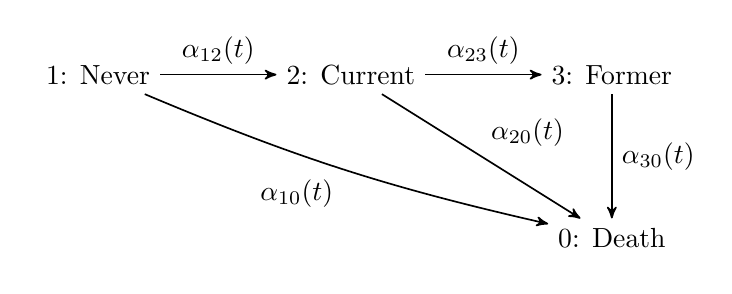
\begin{tikzpicture}[->,bend
  angle=20,semithick,>=stealth']%,font=\sffamily]
\pgfsetmatrixcolumnsep{15mm}
\matrix [matrix of nodes,row sep=16mm,ampersand replacement=\&]
{
|(Never)| 1: Never \& |(Current)| 2: Current  \&
|(Former)| 3: Former \\ %\& |(Reclassified)| 4: Reclassified  \\
 \& \& |(Death)| 0: Death \\
};
\begin{scope}[every node/.style={midway,auto}]
\draw (Never) to node {$\alpha_{12}(t)$} (Current);
\draw (Current) to node {$\alpha_{23}(t)$} (Former);
%\draw (Former) to  node {$\alpha_{34}(t)$} (Reclassified);
\draw (Never) to [bend right=5] node [anchor=north east] {$\alpha_{10}(t)$} (Death);
\draw (Current) to node {$\alpha_{20}(t)$} (Death);
\draw (Former) to node {$\alpha_{30}(t)$} (Death);
%\draw (Reclassified) to  node {$\alpha_{40}(t)$} (Death);
\end{scope}
\end{tikzpicture}
\end{center}
  \caption{Model A for smoking behaviour}
  \label{fig:baseline}
\end{figure}

\begin{figure}[ht]
\begin{center}
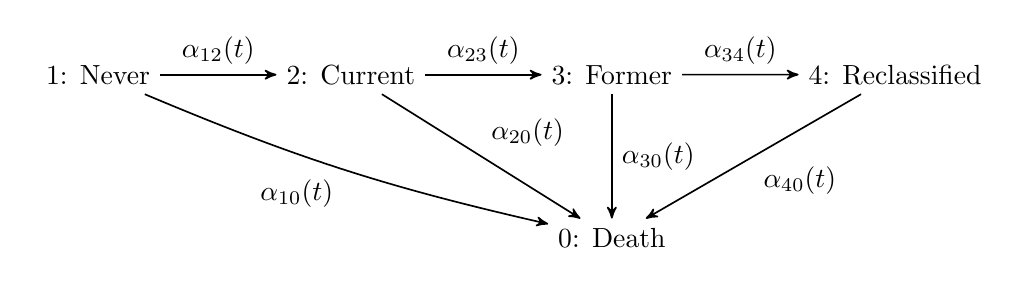
\begin{tikzpicture}[->,bend
  angle=20,semithick,>=stealth']%,font=\sffamily]
\pgfsetmatrixcolumnsep{15mm}
\matrix [matrix of nodes,row sep=16mm,ampersand replacement=\&]
{
|(Never)| 1: Never \& |(Current)| 2: Current  \&
|(Former)| 3: Former \& |(Reclassified)| 4: Reclassified  \\
 \& \& |(Death)| 0: Death \\
};
\begin{scope}[every node/.style={midway,auto}]
\draw (Never) to node {$\alpha_{12}(t)$} (Current);
\draw (Current) to node {$\alpha_{23}(t)$} (Former);
\draw (Former) to  node {$\alpha_{34}(t)$} (Reclassified);
\draw (Never) to [bend right=5] node [anchor=north east] {$\alpha_{10}(t)$} (Death);
\draw (Current) to node {$\alpha_{20}(t)$} (Death);
\draw (Former) to node {$\alpha_{30}(t)$} (Death);
\draw (Reclassified) to  node {$\alpha_{40}(t)$} (Death);
\end{scope}
\end{tikzpicture}
\end{center}
  \caption{Model B for smoking behaviour}
  \label{fig:baselineB}
\end{figure}



Let the probability of moving from state $i$ at time $s$ to state $j$
at time $t$ be $P_{ij}(s,t)$, and define
$\alpha_{ii}(s)=-\sum_{j\neq i} \alpha_{ij}(s)$. Then we have the
Kolmogorov forward differential equations:

\begin{align*}
  P_{ij}(s,s) &= \begin{cases}
    1, & \text{if}\ i=j \\
    0, & \text{otherwise}
  \end{cases} \\
  \frac{\partial P_{ij}(s,t)}{\partial t} &= \sum_k P_{ik}(s,t)
  \alpha_{kj}(t), \qquad s<t
\end{align*}

Given the transition intensities $\alpha_{ij}(t)$ as continuous
functions of time $t$ and initial values $P_{ij}(s,s)$, the transition
probabilities can be calculated using ordinary differential equations
as an initial value problem.  Notably, we propose continuous-time
functions for the transition intensities, rather than
piecewise-constant functions or non-parametric baseline hazard
functions that are typically used for multi-state Markov models.



\section{Survey sampling with recall of behaviour}

If a survey is undertaken at time $\tau$
and an analysis is undertaken retrospectively, then we have a
model that is conditional on being observable, with observed transition
intensity $\lambda_{ij}(t;\tau)$ from state $i$ to state $j$ at time $t$, with observed transition probabilities $Q_{ij}(s,t;\tau)$ from state $i$ at time $s$ to state $j$ at time $t$.

% conditional on observation at time $\tau$ 

\begin{figure}[ht]
  
\begin{center}
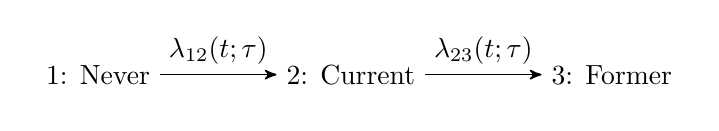
\begin{tikzpicture}[->,bend
  angle=20,semithick,>=stealth'] %,font=\sffamily]
\pgfsetmatrixcolumnsep{15mm}
\matrix [matrix of nodes,row sep=8mm,ampersand replacement=\&]
{
|(Never)| 1: Never  \& |(Current)| 2: Current  \&
|(Former)| 3: Former  \\
};
\begin{scope}[every node/.style={midway,auto}]
\draw (Never) to node {$\lambda_{12}(t;\tau)$} (Current);
\draw (Current) to node {$\lambda_{23}(t;\tau)$} (Former);
\end{scope}
\end{tikzpicture}
\end{center}
  \caption{Observed model for smoking behaviour}
  \label{fig:recall}
\end{figure}

The framework of purged Markov chains by \citet{hoem_purged_1969}
provides theory for when some states are ``purged'' and not observed.
From Hoem and others, it is well known that the observed transition
rates are biased by differential survival. Let $\K$ represent the states that are observable from the survey, and let $P_{i\K}(t,\tau)=\sum_{j \in \K}P_{ij}(t,\tau)$ be the
probability of being in state $i$ at time $t$ and being in an observable state at time
$\tau$. Then
\[
\lambda_{ij}(t;\tau)=\alpha_{ij}(t)\frac{P_{j\K}(t,\tau)}{P_{i\K}(t,\tau)}
\]

% If the probability of being observed conditional on survival is
% independent of state (that is, there is representative sampling), then
% $\Pi_j(t,\tau)/\Pi_i(t,\tau)=(\sum_{k:\
%   \text{alive}}P_{jk}(t,\tau))/(\sum_{k:\
%   \text{alive}}P_{jk}(t,\tau))$.

\noindent and
\[Q_{ij}(s,t;\tau)=P_{ij}(s,t)\frac{P_{j\K}(t,\tau)}{P_{i\K}(s,\tau)}
\]

This result generalises the approach used by
\citet{harris_cigarette_1983} to adjust for the effect of differential
survival when reconstructing smoking prevalence.

The reclassification of former smokers as never smokers is awkward, as the observed and modelled states are no longer one-to-one: observed never smokers comprise never and reclassified smokers in the underlying model. This requires that we differentiate between the observed states and the states for the underlying model; for observed never smokers, the probability is the sum of probabilities for never smokers and reclassified smokers (that is, $Q_{11}(s,t;\tau)+Q_{14}(s,t;\tau)$). The uptake of smoking can now be measured in terms of those who have never been smokers, which is the modelled $\alpha_{12}(s)$, but which is not observable, or in terms of those who presently identify as never being smokers, which would be expressed as $\alpha_{12}(s)\frac{P_{11}(0,s)}{P_{11}(0,s)+P_{14}(0,s)}$. At younger ages, $P_{14}(0,s)$ will be small and the two transition rates will be similar.

Given values of the transition intensities $\alpha_{ij}(t)$, we are
able to calculate $P_{ij}(s,t)$, $P_{i\K}(t,\tau)$,
$\lambda_{ij}(t;\tau)$ and $Q_{ij}(s,t;\tau)$ for any values of
$i,j,s,t$ and $\tau$.  In particular, given the intensities for the
underlying model, we are able to calculate the transition intensities
and transition probabilities for the observed survey data, which supports estimation of the underlying intensities using the likelihood for the observed data.

\subsection{Some theoretical considerations}

The proposed Model A is progressive and is a Coxian phase-type distribution with nonhomogeneous (time-dependent) transition intensities.

\begin{theorem}
For a purged Markov model, consider an observation that starts in state $u_1$ at time $t_1$ and is observed in state $v_I$ at time $\tau$ with intervals $[t_i,t_{i+1})$ being in state $u_i$ at time $t_i$ and state $v_i$ at time $(t_{i+1}-)$ with an observed transition from state $v_i$ to state $u_{i+1}$ at time $t_{i+1}$. Then the density of the observation is

\begin{align*} 
\prod_{i=1}^{I-1} \left\{Q_{u_i,v_i}(t_i,t_{i+1};\tau) \lambda_{v_i,u_{i+1}}(t_{i+1};\tau)\right\}Q_{u_I,v_I}(t_I,\tau;\tau)
= \frac{\prod_{i=1}^{I-1} \left\{P_{u_i,v_i}(t_i,t_{i+1}) \alpha_{v_i,u_{i+1}}(t_{i+1})\right\}P_{u_I,v_I}(t_I,\tau)}{P_{u_1,K}(t_1,\tau)}
\end{align*}
\end{theorem}

\begin{proof}
\begin{align*} 
& \prod_{i=1}^{I-1} \left\{Q_{u_i,v_i}(t_i,t_{i+1};\tau) \lambda_{v_i,u_{i+1}}(t_{i+1};\tau)\right\}Q_{u_I,v_I}(t_I,\tau;\tau)\\
= & \prod_{i=1}^{I-1} \left\{P_{u_i,v_i}(t_i,t_{i+1})\frac{P_{v_i,K}(t_{i+1},\tau)}{P_{u_i,K}(t_{i},\tau)} \alpha_{v_i,u_{i+1}}(t_{i+1})\frac{P_{u_{i+1},K}(t_{i+1},\tau)}{P_{v_i,K}(t_{i+1},\tau)}\right\}\frac{P_{u_I,v_I}(t_I,\tau)}{P_{u_I,K}(t_{I},\tau)} \\
 = & \prod_{i=1}^{I-1} \left\{P_{u_i,v_i}(t_i,t_{i+1})\alpha_{v_i,u_{i+1}}(t_{i+1})\right\} 
\frac{P_{u_I,v_I}(t_I,\tau)}{P_{u_I,K}(t_{I},\tau)}
 \prod_{i=1}^{I-1} \frac{P_{u_{i+1},K}(t_{i+1},\tau)}{P_{u_i,K}(t_{i},\tau)} \\
 = & \prod_{i=1}^{I-1} \left\{P_{u_i,v_i}(t_i,t_{i+1})\alpha_{v_i,u_{i+1}}(t_{i+1})\right\} 
\frac{P_{u_I,v_I}(t_I,\tau)}{P_{u_1,K}(t_{1},\tau)}
\end{align*}
\end{proof} 

\section{Data sources}

% Yes, we have great data...

Individual-level data were available from respondents to smoking questions from the National Health Interview Surveys from 1965 to 2010. In total, there were 1,000,387 respondents. 

The main data requirements are accurate estimates of the mortality
rate functions by age, sex, calendar period and smoking
status\footnote{As a possible model extension, the smoking model could
  be expanded to include states by smoking dose.}  . The current
smoking history generator only includes differential mortality by ever
versus never smokers, while the proposed model would need these rates
for never, current and former smokers.

The current smoking history generator is also based on unweighted
survey data. Survey weights and any other survey data, such as primary
sampling unit, would improve the validity of the estimates. 

\begin{figure}[ht]
  \centering
  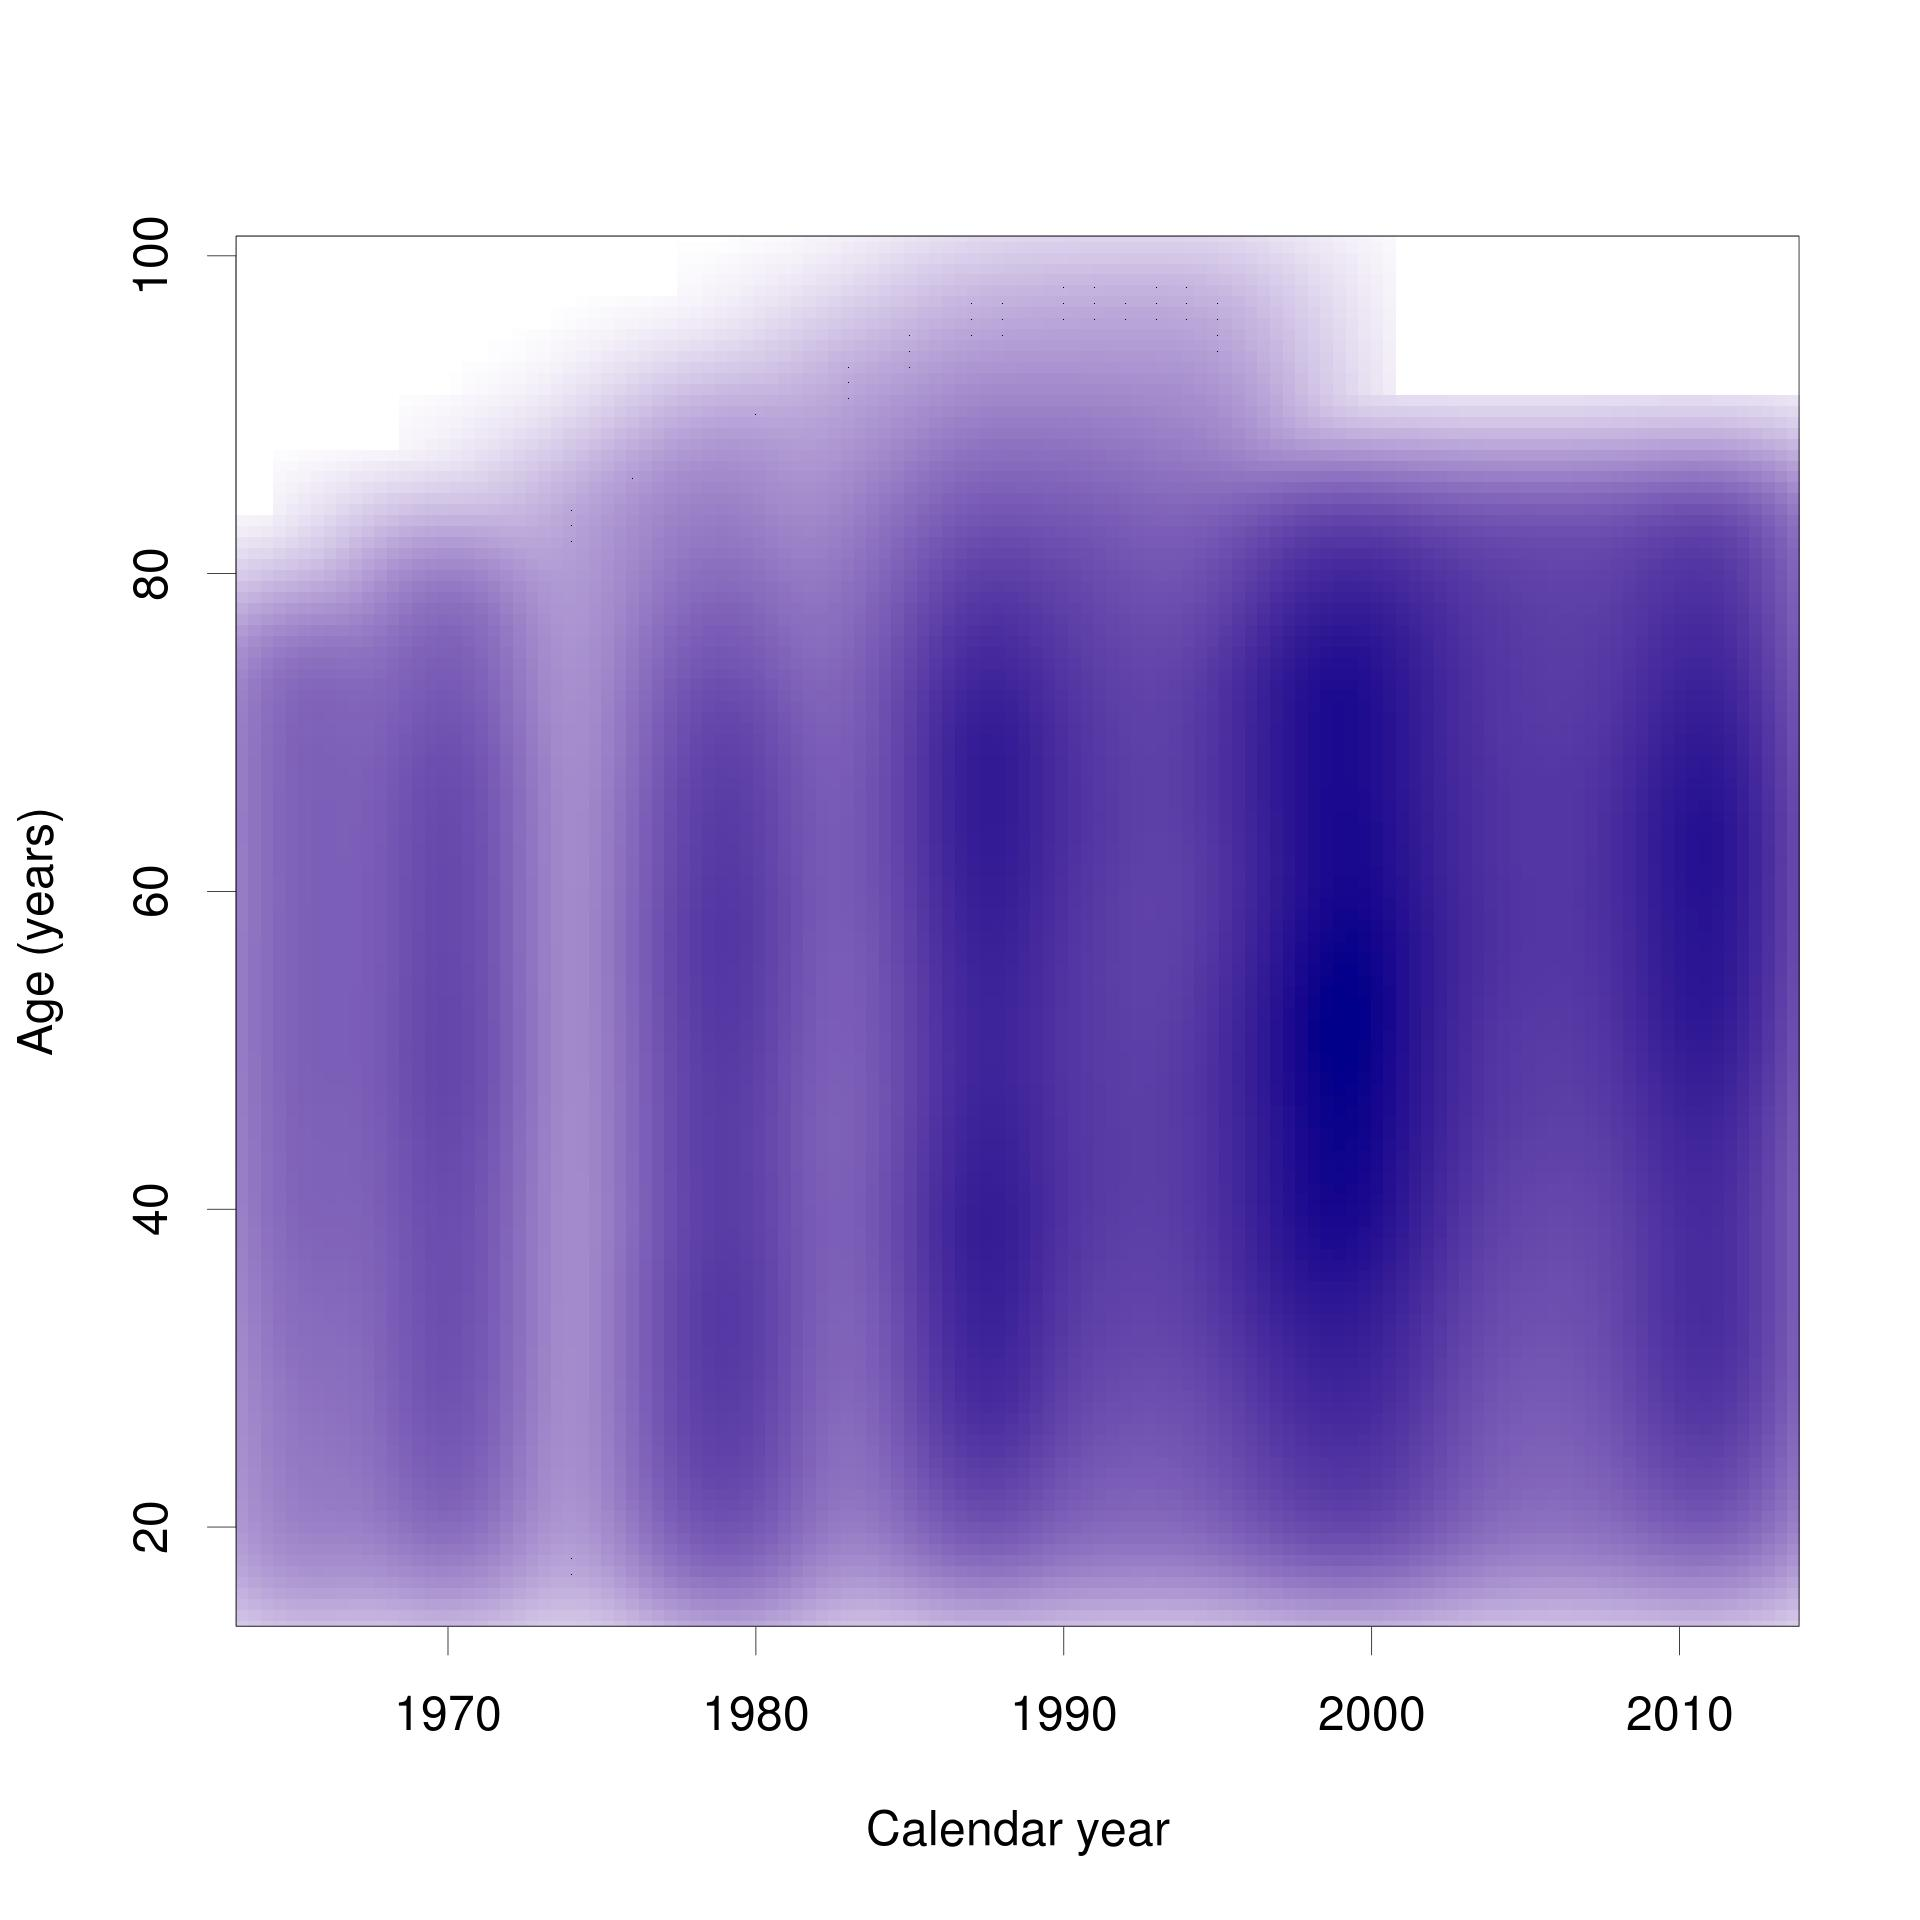
\includegraphics[width=0.6\textwidth]{nhis_density.jpg}    
  \caption{Density plot for respondents to the NHIS surveys, by age and calendar period, 1965--2011.}
  \label{fig:nhis}
\end{figure}


\section{Likelihood}

The likelihood components for observed data are available for six
different forms of data: current status for (i) never, (ii) current
and (iii) former smokers, and recalled behaviour for (iv) current
smokers, (v) former smokers with time of uptake and cessation, and
(vi) former smokers with time of cessation only.  

The likelihood component $L$ for an observed never smoker is, given the underlying system, the 
probability for a never smoker and the probability for a reclassified smoker, such that
\begin{align*}
  %\label{eq:Lnever}
L_1(\tau) & = Q_{11}(0,\tau;\tau)+Q_{14}(0,\tau;\tau) \\
& = P_{11}(0,\tau)\frac{P_{1\K}(\tau,\tau)}{P_{1\K}(0,\tau)} +P_{14}(0,\tau)\frac{P_{4\K}(\tau,\tau)}{P_{1\K}(0,\tau)} 
= \frac{P_{11}(0,\tau)+P_{14}(0,\tau)}{P_{1\K}(0,\tau)}  
\end{align*}

In this case, the likelihood based on current status and recalled information are the same.
For current smokers who have recalled information on age $s$ that they started smoking,

\begin{align*}
L_{12}(s,\tau) & = Q_{11}(0,s;\tau)\lambda_{12}(s;\tau)Q_{22}(s,\tau;\tau) \\
& = P_{11}(0,s)\frac{P_{1\K}(s,\tau)}{P_{1\K}(0,\tau)} 
\alpha_{12}(s) \frac{P_{2\K}(s,\tau)}{P_{1\K}(s,\tau)}
P_{22}(s,\tau)\frac{P_{2\K}(\tau,\tau)}{P_{2\K}(s,\tau)}
 = \frac{P_{11}(0,s)\alpha_{12}(s)P_{22}(s,\tau)}{P_{1\K}(0,\tau)}
\end{align*}

For current smokers who only have information on their current status, 

\begin{align*}
L_2(\tau) & = Q_{12}(0,\tau;\tau)  = P_{12}(0,\tau)\frac{P_{2\K}(\tau,\tau)}{P_{1\K}(0,\tau)} 
= \frac{P_{12}(0,\tau)}{P_{1\K}(0,\tau)}  
\end{align*}

For former smokers who have recalled information on age $s$ that they started smoking and age $t$ that they quit smoking,

\begin{align*}
L_{123}(s,t,\tau) & = Q_{11}(0,s;\tau) \lambda_{12}(s;\tau) Q_{22}(s,t;\tau) \lambda_{23}(t;\tau) Q_{33}(t,\tau;\tau) \\
& = P_{11}(0,s)\frac{P_{1\K}(s,\tau)}{P_{1\K}(0,\tau)} 
\alpha_{12}(s) \frac{P_{2\K}(s,\tau)}{P_{1\K}(s,\tau)}
P_{22}(s,t)\frac{P_{2\K}(t,\tau)}{P_{2\K}(s,\tau)}
\alpha_{23}(t) \frac{P_{3\K}(t,\tau)}{P_{2\K}(t,\tau)}
P_{33}(t,\tau)\frac{P_{3\K}(\tau,\tau)}{P_{3\K}(t,\tau)} \\
& = \frac{P_{11}(0,s) \alpha_{12}(s) P_{22}(s,t) \alpha_{23}(t) P_{33}(t,\tau)}{P_{1\K}(0,\tau)}
\end{align*}

For former smokers who only have information on their current status, 

\begin{align*}
L_3(\tau) & = Q_{13}(0,\tau;\tau)  = P_{13}(0,\tau)\frac{P_{3\K}(\tau,\tau)}{P_{1\K}(0,\tau)} 
= \frac{P_{13}(0,\tau)}{P_{1\K}(0,\tau)}  
\end{align*}

For the final likelihood component, some respondents who were former smokers only had information on the age that they quit smoking, thus
 
\begin{align*}
L_{23}(t,\tau) & = Q_{12}(0,t;\tau) \lambda_{23}(t;\tau) Q_{33}(t,\tau;\tau) \\
& = P_{12}(0,t)\frac{P_{2\K}(t,\tau)}{P_{1\K}(0,\tau)} 
\alpha_{23}(t) \frac{P_{3\K}(t,\tau)}{P_{2\K}(t,\tau)}
P_{33}(t,\tau)\frac{P_{3\K}(\tau,\tau)}{P_{3\K}(t,\tau)} \\
& = \frac{P_{12}(0,t) \alpha_{23}(t) P_{33}(t,\tau)}{P_{1\K}(0,\tau)}
\end{align*}

The likelihood components can be recognised as the standard
multi-state model likelihoods conditional on being observable.  Let the data
be stratified into disjoint sets $\Omega_k$, where $k$ represents the
available data. Then the total likelihood is equal to
\begin{align*}
  L = 
\prod_{i \in \Omega_1} L_1(\tau_i)  
\prod_{i \in \Omega_2} L_2(\tau_i)  
\prod_{i \in \Omega_3} L_3(\tau_i)  
\prod_{i \in \Omega_{12}} L_{12}(s_i,\tau_i)  
\prod_{i \in \Omega_{123}} L_{123}(s_i,t_i,\tau_i)  
\prod_{i \in \Omega_{23}} L_{23}(t_i,\tau_i)  
\end{align*}


\section{Estimation}

The mortality intensity functions $\alpha_{10}(t)$, $\alpha_{20}(t)$
and $\alpha_{30}(t)$ were available. We also assumed that the
mortality rates for reclassified smokers were the same as for never
smokers (that is, $\alpha_{40}(t)=\alpha_{10}(t)$). We estimated
parameters for $\alpha_{12}(t)$ and $\alpha_{23}(t)$ would be
estimated. Moreover, for multiple surveys, parameters for
$\alpha_{34}(t)$ was estimated.

The likelihood was optimised using the Nelder-Mead algorithm, with variance estimates calculated using the inverse of the Hessian matrix.

% We propose using maximum penalised likelihood to investigate the
% likelihood function, using p-splines to investigate the functional
% forms for $\alpha_{12}(t)$, $\alpha_{23}(t)$ and
% $\alpha_{34}(t)$. 

% discrete time: multinomial outcome? It also leads to methods for
% analysis of grouped data.

\section{Implementation}

As the transition probabilities need to be recalculated for each
update of parameters, we chose to implement the model using a compiled
language. Specifically, we implemented the model in C, using an
ordinary differential equation solver from the GNU Scientific Library
(GSL; see Appendix). As the values of $t$ are not fixed in advanced,
the basis functions for $\alpha_{ij}(t)$ need to be calculated in C
code.  We have implemented the functional forms for the initiation and
cessation rates using penalised B-splines with equidistant knots
(``p-splines''). These spline functions were implemented in C using
the GSL.  The C code was linked to R for optimising the likelihood and
for post-estimation.  The implementation does not currently offer
automatic selection of the smoothing parameters, where selection would
be based on an approximate cross-validation criterion
\cite[e.g.][]{joly_penalized_2002,cai_hazard_2003}.

The model development has focused on cohort-specific transition rates.
In practice, data from multiple birth cohorts would be modelled
together across the Lexis diagram. A simple solution would be to model
the rates using age-period models. A better solution would be to model
the rates across the Lexis diagram using tensor product splines.
The specification of the transition rates across the Lexis diagram
will also allow for the investigation of future smoking prevalence
under different scenarios for future smoking uptake and cessation rates.


\section{Results}

\begin{figure}[ht]
  \centering
  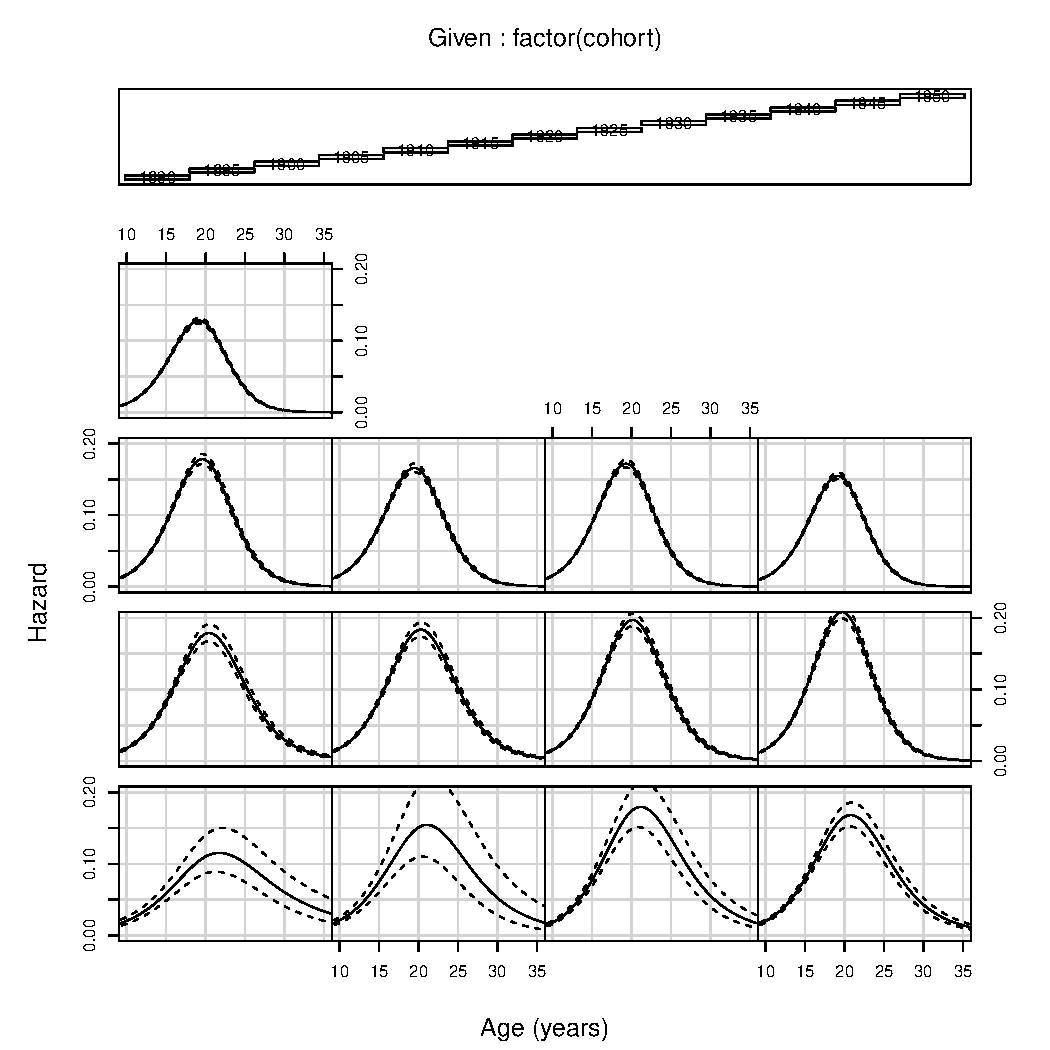
\includegraphics[width=0.6\textwidth]{coplot-1.pdf}    
  \caption{Smoking initiation rates, NHIS, males}
  \label{fig:init-males}
\end{figure}
\begin{figure}[ht]
  \centering
  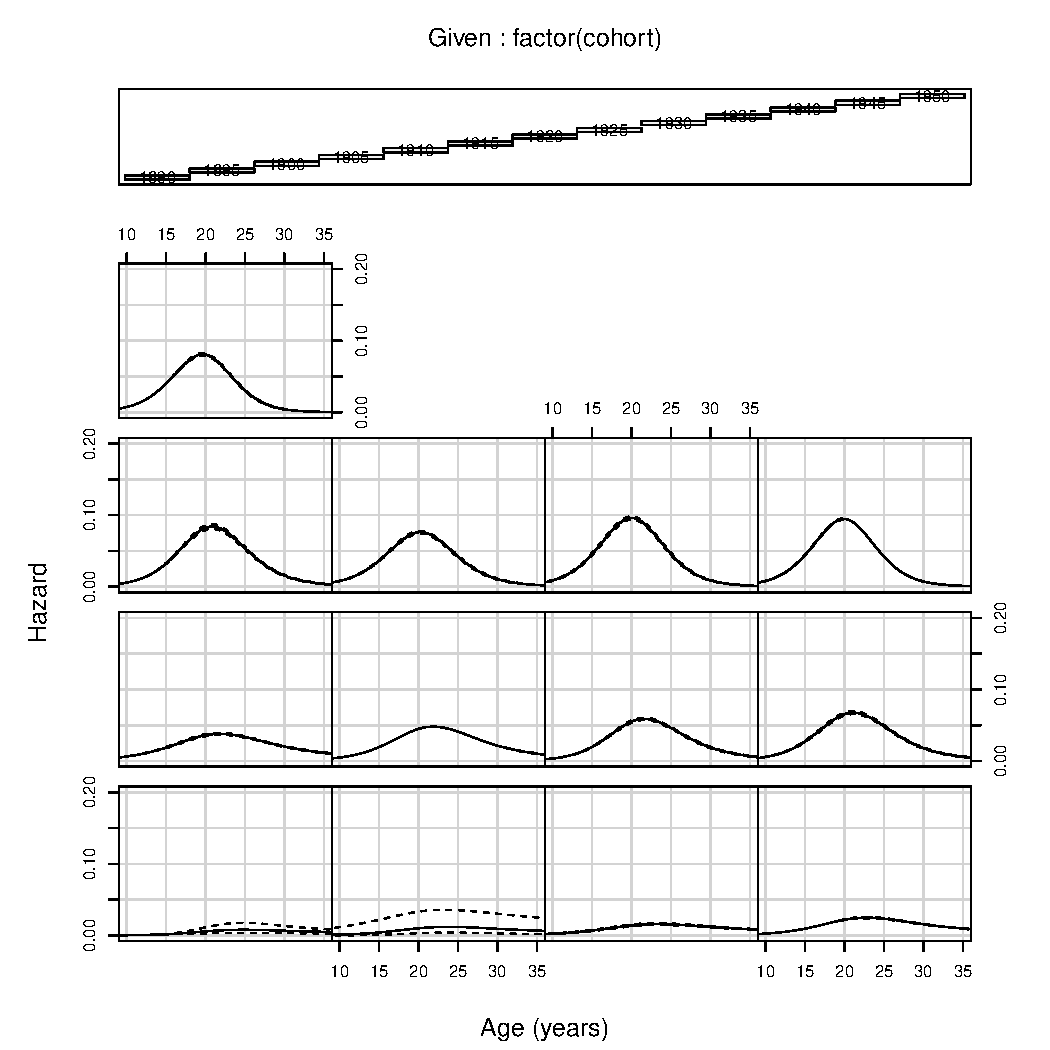
\includegraphics[width=0.6\textwidth]{coplot-2.pdf}    
  \caption{Smoking initiation rates, NHIS, females}
  \label{fig:init-females}
\end{figure}
\begin{figure}[ht]
  \centering
  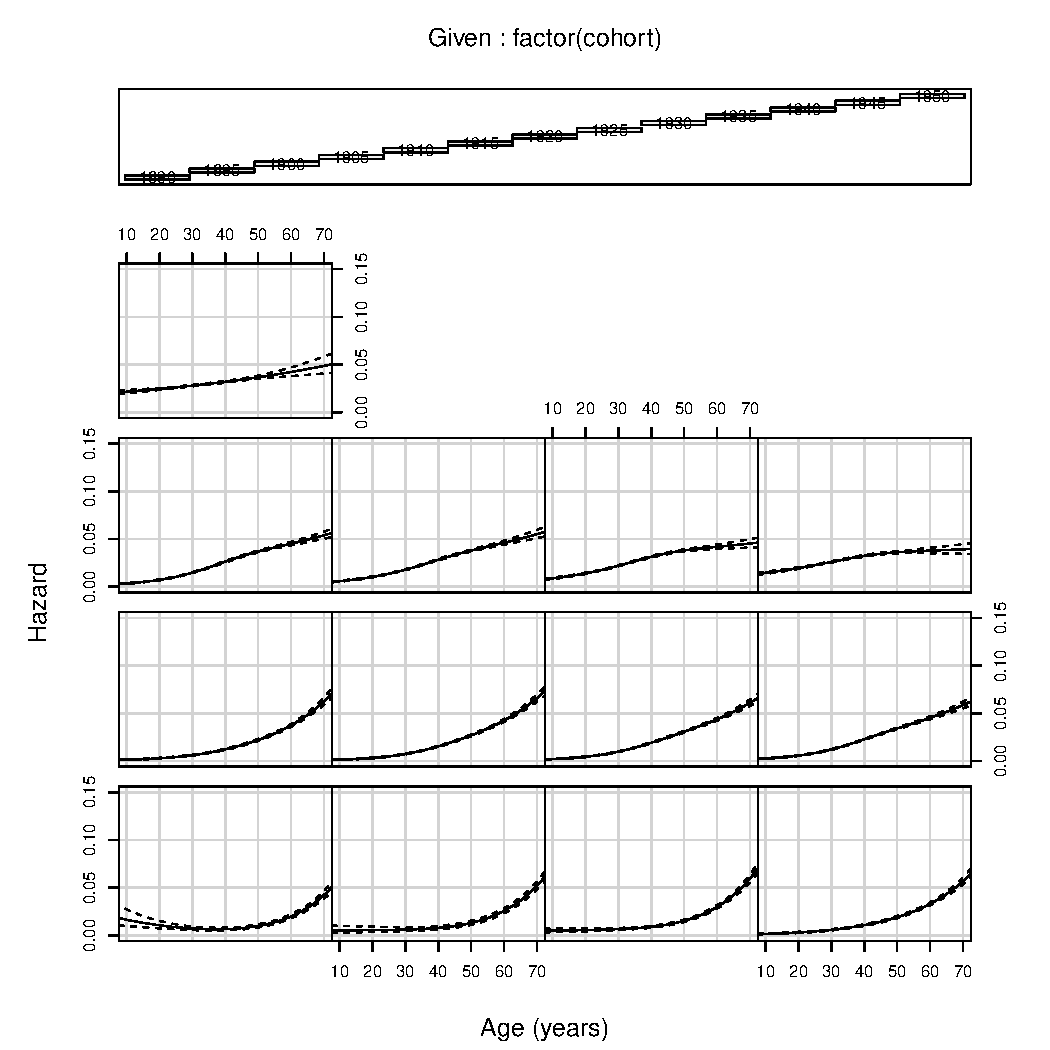
\includegraphics[width=0.6\textwidth]{coplot-3.pdf}    
  \caption{Smoking cessation rates, NHIS, males}
  \label{fig:cess-males}
\end{figure}
\begin{figure}[ht]
  \centering
  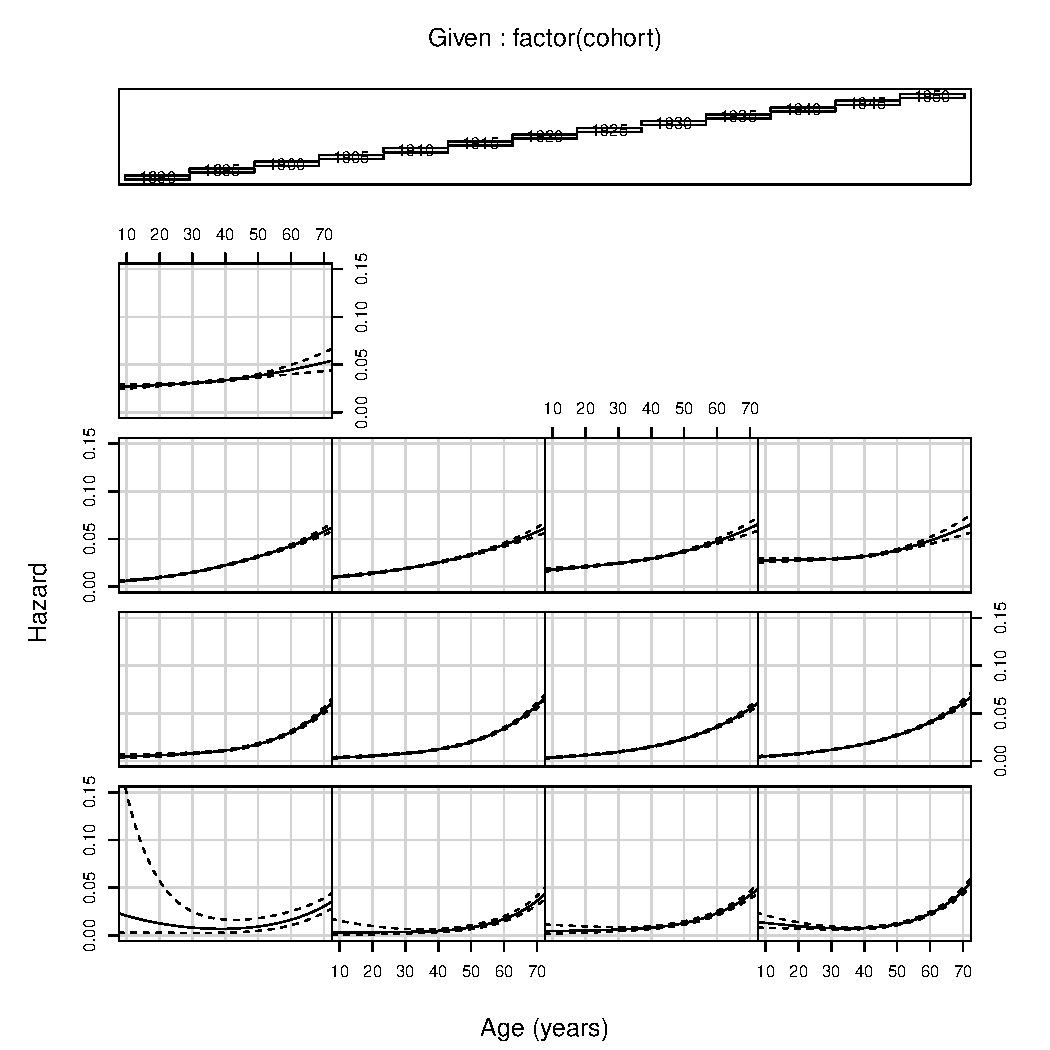
\includegraphics[width=0.6\textwidth]{coplot-4.pdf}    
  \caption{Smoking cessation rates, NHIS, females}
  \label{fig:cess-females}
\end{figure}



\bibliography{research-prostate-2012_zotexo_}
% \bibliography{mylib}

\end{document}

% Local Variables:
% zotero-collection: #("0" 0 1 (name "*ALL*"))
% End:
